\documentclass[11pt,a4paper]{article}

\usepackage[margin=2.5cm]{geometry}
\usepackage{amsmath,amssymb,amsthm}
\usepackage{mathtools}
\usepackage{bm}
\usepackage{hyperref}
\usepackage{graphicx}
\providecommand{\rotatebox}[2]{#2} % pandoc fallback (LaTeX ignores — already defined by graphicx)
\usepackage{booktabs}
\usepackage{microtype}
\usepackage{parskip}
\usepackage{natbib}
\usepackage{comment}

% ---- web-only collapsible (hidden from PDF, becomes <details> on web) ----
\excludecomment{weboptional}

% ---- notes (visible in PDF, collapsible on web) ----
% Optional arg = summary label (may contain inline formatting). Default: "Notes".
\newenvironment{notes}[1][Notes]{%
  \par\vspace{0.2em}#1:%
  \begin{itemize}%
}{%
  \end{itemize}%
}

% ---- experiments (nested under a hypothesis / proposal; same treatment both outputs) ----
\newenvironment{experiments}[1][Experiments]{%
  \par\vspace{0.2em}#1\par\vspace{0.1em}%
}{%
  \par%
}

% ---- figure grid trim (bp) ----
\newlength{\cropL}\setlength{\cropL}{20bp}   % left crop for inner columns
\newlength{\cropLfirst}\setlength{\cropLfirst}{0bp}  % left crop for leftmost column (keep y-axis)
\newlength{\cropB}\setlength{\cropB}{0bp}    % bottom crop for bottom row
\newlength{\cropBtop}\setlength{\cropBtop}{20bp}  % bottom crop for top row (remove x-axis)
\newlength{\cropR}\setlength{\cropR}{0bp}    % right crop
\newlength{\cropT}\setlength{\cropT}{20bp}   % top crop

% ---- notation shortcuts ----
\newcommand{\R}{\mathbb{R}}
\newcommand{\E}{\mathbb{E}}
\newcommand{\tr}{\operatorname{tr}}
\newcommand{\kron}{\otimes}
\DeclareMathOperator*{\argmin}{arg\,min}

\title{\textbf{What Happens Inside a Language Model as it Trains?}\\[0.4em]}
\author{Dante Campregher}
\date{\today}

\begin{document}
\maketitle

% =========================================================
\section{Introduction}
% =========================================================

When a language model trains, its weights change, but the raw weight matrices are hard to interpret.
A more revealing approach is to look at the \emph{activations}: the vectors that flow through the network when it processes text.
If we collect enough of these vectors, we can ask what their distribution looks like and how that distribution changes over the course of training.

This post describes a set of experiments that do exactly that.
We collect covariance matrices of activations (and gradients) at specific locations inside the network, decompose them into eigenvectors and eigenvalues, and track the resulting eigenvalue spectra from random initialisation through to convergence.

I was inspired by the work of \citet{li2025tracing}, who traced the Entropy of the covariance of final tokens of documents. In this post, we reproduce their work and dig deeper into the training dynamics that cause the macroscopic changes we see. For using K-FAC to estimate curvature in language models, I was inspired by \citet{merullo2025memorization}.

We work with two families of open-weight language models:
\begin{itemize}
  \item \textbf{Pythia}: GPT-style models from 14M to 12B parameters, trained on the Pile.
  \item \textbf{OLMo-2}: 1B and 7B parameter models with a LLaMA-style architecture, trained on OLMo-Mix.
\end{itemize}

Both families release intermediate checkpoints, which is what makes this kind of analysis possible.
Various quantities we use are:
\begin{enumerate}
  \item \textbf{RankMe}: roughly how many directions of the representation space are being occupied by the data.
  \item \textbf{$\alpha$-ReQ}: how quickly the eigenvalue spectrum decays — the power-law exponent.
  \item \textbf{K-FAC log-determinant}: a measure of how curved the loss landscape is near each layer's weights. Specifically: the \emph{log-volume} of the curvature.
  \item \textbf{Mean fraction of total energy}: how much of the uncentered covariance is attributed to the mean of the data.
  % \item \textbf{Mean alignment with covariance}: how much the mean lies in the same direction as the uncentered covariance.
\end{enumerate}

The specifics of each will be elaborated on in Section~\ref{sec:metrics}.

% =========================================================
\section{Background: covariance matrices and their spectra}
% =========================================================

\subsection{Covariance matrices from activations}

Consider passing a large batch of text through the model and recording the activation vector $\mathbf{x} \in \R^d$ at some fixed point in the network (say, the input to a particular layer) for every token position.
This gives $N$ vectors $\mathbf{x}_1, \dots, \mathbf{x}_N \in \R^d$, which we stack as rows of a matrix $\mathbf{X} \in \R^{N \times d}$.

The standard way to summarise this cloud of points is through its covariance matrix.
We use two versions:

\paragraph{Uncentered covariance.} The average outer product of the raw activations:
\begin{equation}
  \bm{\Sigma}_A = \frac{1}{N}\mathbf{X}^\top \mathbf{X} \in \R^{d\times d}.
\end{equation}
This captures both the direction of the mean activation and the spread around it.

\paragraph{Centered covariance.} Here we subtract the mean first, isolating the spread:
\begin{equation}
  \hat{\bm{\Sigma}}_A = \bm{\Sigma}_A - \bm{\mu}\bm{\mu}^\top, \qquad \bm{\mu} = \frac{1}{N}\sum_{i=1}^N \mathbf{x}_i.
\end{equation}

The difference between centered and uncentered covariance matters. Namely, If the mean is large, the uncentered covariance will be dominated by one direction, even if the actual variation is distributed across dimensions.

We eigendecompose $\hat{\bm{\Sigma}}_A = \mathbf{V}\bm{\Lambda}\mathbf{V}^\top$, giving eigenvalues $\lambda_1 \ge \lambda_2 \ge \cdots \ge \lambda_d \ge 0$.
The sorted $\lambda$ together make up the \emph{eigenspectrum}, which is the central object of this analysis.

\subsection{Gradient covariance}

Besides forward activations, we also collect \emph{gradient} signals.
For an MLP weight matrix $\mathbf{W}$, the curvature of the loss is usually captured by the Hessian $\mathbf{H} = \nabla_\theta^2 L(\theta)$. Where L is the loss and $\theta$ is the flattened parameters $\mathbf{W}$. The Hessian itself is intractable for any large model, but it can be approximated by the Fisher Information Matrix.
Under the K-FAC approximation \citep{martens2020optimizing}, this factorises as a Kronecker product:
\begin{equation}
  \mathbf{F}_{\mathbf{W}} \approx \bm{\Sigma}_G \kron \bm{\Sigma}_A,
\end{equation}
where $\bm{\Sigma}_A$ is the (uncentered) input activation covariance and $\bm{\Sigma}_G$ is the gradient covariance:
\begin{equation}
  \bm{\Sigma}_G = \frac{1}{N}\mathbf{G}^\top \mathbf{G},
\end{equation}
with $\mathbf{G} \in \R^{N \times d}$ the matrix of per-sample gradients of the loss with respect to the \emph{pre-activation output of the layer}.
$\bm{\Sigma}_A$ tells us which input directions are active; $\bm{\Sigma}_G$ tells us which output directions receive strong gradient signal.
Together, they describe the curvature structure of the loss around each layer's weights.

To collect $\bm{\Sigma}_G$ we use \emph{sampled labels}: we sample from the model's own output distribution and backpropagate through those samples rather than the true labels.
This gives an unbiased estimate of the Fisher information.

% =========================================================
\section{Metrics}\label{sec:metrics}
% =========================================================

\subsection{RankMe: how many dimensions are being used?}

If all the variance in a representation is concentrated in a single direction, the covariance matrix is effectively rank-1.
If variance is spread uniformly across all $d$ dimensions, the matrix has full rank.
RankMe \citep{garrido2023rankme} quantifies where a representation sits between these extremes, using the entropy of the normalised eigenvalue distribution:
\begin{equation}
  p_i = \frac{\lambda_i}{\sum_j \lambda_j}, \qquad
  \text{RankMe} = \exp\!\left(-\sum_i p_i \log p_i\right).
\end{equation}
The result is always between 1 and $d$.
Values near 1 indicate that one eigenvalue dominates; values near $d$ indicate a roughly uniform spectrum.

The eigenvalues $\lambda_i$ are conventionally the eigenvalues of the centered covariance. We follow this convention unless otherwise stated.

The original RankMe paper normalises by singular values $\sigma_i = \sqrt{\lambda_i}$ rather than eigenvalues, which gives slightly different results.
We compute both, but to remain consistent with \citet{li2025tracing}, we focus on the eigenvalue RankMe.

\subsection{Power-law exponent \texorpdfstring{$\alpha$}{alpha}: how fast does the spectrum decay?}

Eigenspectra of neural network layers are rarely flat.
They tend to follow a power law:
\begin{equation}
  \lambda_i \approx C \cdot i^{-\alpha}.
\end{equation}
On a log-log plot this is a straight line with slope $-\alpha$.
Larger $\alpha$ means steeper decay: only a few directions matter.
Smaller $\alpha$ means many dimensions contribute.

We fit $\alpha$ by weighted least-squares following \citet{stringer2019highdimensional}, using weights $w_i = 1/i$ so that the leading (most reliable) eigenvalues carry more influence:
\begin{equation}
  \hat\alpha = \argmin_\alpha \sum_{i} \frac{1}{i} \bigl(\log\lambda_i + \alpha\log i - \log C\bigr)^2.
\end{equation}
% $R^2$ is reported as a quality-of-fit indicator.

\subsection{K-FAC log-determinant}

Under Kronecker-factored Approximate Curvature (K-FAC) Fisher $\mathbf{F}_{\mathbf{W}}$ is approximated as $\bm{\Sigma}_G \kron \bm{\Sigma}_A$, the eigenvalues of the full matrix for a weight $\mathbf{W}$ are the pairwise products $\{\lambda^G_j \lambda^A_i\}$.
A useful scalar summary is the log-determinant, which measures the log-volume of the curvature ellipsoid.

To maintain numerical stability for logs of near-zero eigenvalues. We compute a damped version, adding a small diagonal term proportional to the trace to avoid numerical issues near zero:
\begin{equation}
  \mathcal{L} = d_\text{in} \cdot \log\det(\bm{\Sigma}_G + \varepsilon_G \mathbf{I}) + d_\text{out} \cdot \log\det(\bm{\Sigma}_A + \varepsilon_A \mathbf{I}),
\end{equation}
where $\varepsilon_G = \alpha \cdot \tr(\bm{\Sigma}_G)/d_\text{out}$ and $\varepsilon_A = \alpha \cdot \tr(\bm{\Sigma}_A)/d_\text{in}$ (with $\alpha = 10^{-6}$).

A larger log-determinant indicates stronger curvature around that layer's weights.

% We also examine the joint eigenspectrum directly: the top-20,000 products $\lambda^A_i \lambda^G_j$ sorted in descending order, which shows which input-output direction pairs dominate the curvature.

\subsection{Mean fraction of total energy}

Although RankMe measures the signal around the mean. The weights along with approximations of their curvature depend on the uncentered covariance. To quantify the potential influence of the mean, we track the mean vector $\bm{\mu}$ of the activations alongside the other spectral metrics. When the mean of the activations is large, the distinction between centered and uncentered covariance becomes important.

We track how much of the total signal energy — that is: the uncentered covariance — sits in the mean versus the variation around it:
\begin{equation}
  \rho_\mu = \frac{\|\bm{\mu}\|^2}{\tr(\bm{\Sigma}_A)}.
\end{equation}
When $\rho_\mu$ is close to 1, nearly all the energy is in the mean (the activations cluster tightly around a point far from the origin).
When $\rho_\mu$ is close to 0, the mean is negligible.
% This matters particularly for OLMo-2, where RMSNorm constrains the scale of activations and tends to inflate $\rho_\mu$.

% \subsection{TODO: Hutchinson trace estimator}

% \subsection{Generalised eigendecomposition}

% For layers where we have both $\bm{\Sigma}_G$ (gradient covariance at the output) and $\bm{\Sigma}_B$ (activation covariance at the output), we can ask which output directions have high gradient variance \emph{relative to} their activation variance.
% This is captured by the generalised eigenvalue problem:
% \begin{equation}
%   \bm{\Sigma}_G \mathbf{v} = \lambda \bm{\Sigma}_B \mathbf{v}.
% \end{equation}
% Directions with large $\lambda$ are those where the optimisation signal is large compared to the typical activation, i.e.\ the directions the optimiser is updating most aggressively.

% =========================================================
\section{Experimental setup}
% =========================================================

\subsection{Models and checkpoints}

\begin{table}[ht]
  \centering
  \caption{Model families studied.}
  \label{tab:models}
  \begin{tabular}{llcc}
    \toprule
    Family & Architecture & Sizes we study & Pretraining Set \\
    \midrule
    Pythia & GPT-NeoX & 1B, 6.9B & The Pile deduped \\
    OLMo-2 & LLaMA-style & 1B, 7B & OLMo-Mix \\
    \bottomrule
  \end{tabular}
\end{table}

Both models provide densely logarithmically spaced checkpoints at the beginning, and constantly spaced checkpoints after that.

For both models we sample all densely spaced early checkpoints, and then 20 square-root spaced checkpoints. Resulting in collecting between and 27 and 36 checkpoints across the four models we measure.

\subsection{Where in the network do we collect?}

We hook into three locations:

\paragraph{Final residual stream.}
The vector that feeds into the unembedding head, captured before and after the final layer norm.
This is the model's final embedding representation for the predicted token. When hooking only after the final norm.

\paragraph{MLP projections.}
Inside each transformer block, the MLP contains two or three weight matrices.
Pythia has two (up and down projections); OLMo-2 has three (gate, up, and down).
We collect activation covariances at the input and output of each projection, and gradient covariances at the outputs.

\subsection{Data}

To reproduce the RankMe experiments of \citet{li2025tracing}, we process 5,000 padded sequences between 32 and 512 tokens long from the fineweb dataset. We then sample the final token of each sequence, giving one representation that summarises the sequence.

For our other experiments we sample 6 million tokens (~45.8MB) from packed and shuffled chunks of the respective pretraining mixes of the models. Measuring all but the first 32 tokens for each chunk. Sampling the full token sequence lets us accumulate vastly more sampled gradients economically.

\subsection{Accumulation}

When capturing only the final token, it is economical to store the activation embeddings themselves, but this quickly becomes infeasible when collecting millions of tokens instead of thousands. To do this, we accumulate covariance matrices by summing the rank one projections of the activations. Storing a matrix of size $d \times d$ where d is the embedding dimension at that hook. This can be cheap in the residual stream. But inside MLPs, the embedding dimension is often 4 times the residual's dimension, presenting a tricky storage-compute dilemma if experiments need to be recomputed.

Covariance matrices are accumulated in \texttt{float64} for numerical stability after millions of accumulations; activations are cast from lower precision to \texttt{float32} before forming outer products.

% =========================================================
\section{Findings}
% =========================================================

\subsection{Reproducing \texorpdfstring{\citet{li2025tracing}}{Li et al. (2025)}}

Reproducing The final layer RankMe with the training dataset shows that the shape of the plot remains consistent, and the entropy- and compression seeking curves are in fact much more pronounced on the model's training set.

\begin{figure}[ht]
  \centering
  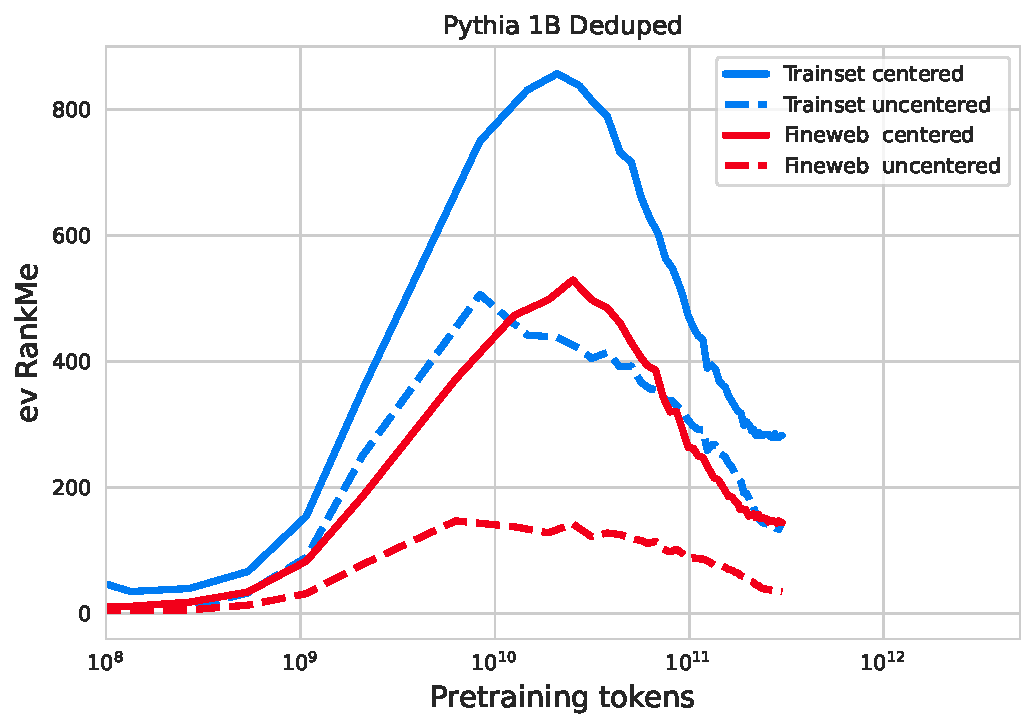
\includegraphics[width=0.48\linewidth]{attachments/li_reproduction/rankme_Pythia_1B_Deduped.pdf}
  \hfill
  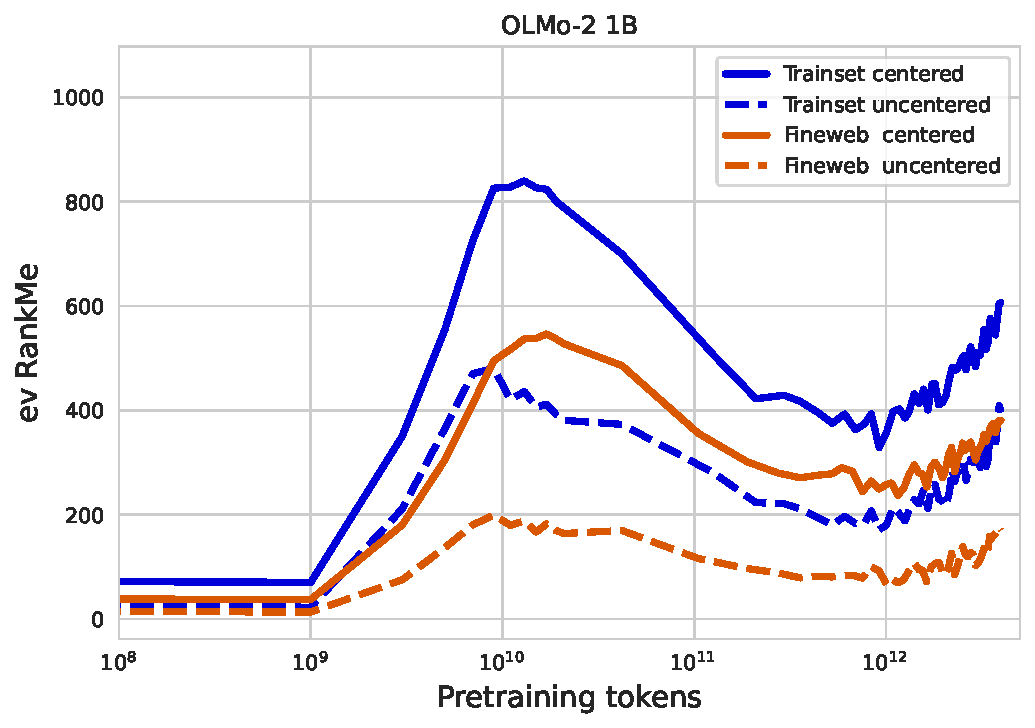
\includegraphics[width=0.48\linewidth]{attachments/li_reproduction/rankme_OLMo-2_1B.pdf}
  \caption{Final residual RankMe over training, comparing the model's training set against FineWeb, with centered and uncentered covariance. The entropy-seeking and compression-seeking phases are more pronounced on the training set.}
  \label{fig:rankme_trainset}
\end{figure}

Unfortunately, although the shape of the plot is consistent with that of \citet{li2025tracing}, we report a lower peak RankMe value for fineweb than they do, using the same setup that they do.

\subsection{How is the residual stream's geometry formed within the model?}

The residual stream at its final point is of course the sum of the output of every block in the model. So does every one of these blocks also output the same pattern, or are the entropy-seeking and compression-seeking phases at the final point of the residual formed through a complex interaction between the signals added.

Since we collected MLP data for K-FAC, we now have MLP down-projection outputs, resembling what will be added to the residual stream. Although, for OLMo-2 models, these activations first go through an RMSNorm before being added to the residual stream. We could capture the activations after the RMSNorm in the future.

Looking at the RankMe statistics of these activations shows that they surprisingly do not generally share the compression-seeking phase of the final residual.

\begin{figure}[ht]
  \centering
  \newlength{\gridimg}\setlength{\gridimg}{0.23\linewidth}%
  \setlength{\tabcolsep}{2pt}
  \begin{tabular}{@{}c@{\hspace{2pt}} cccc@{}}
    & \small Pythia-1B & \small Pythia-6.9B & \small OLMo-2-1B & \small OLMo-2-7B \\[2pt]
    \rotatebox{90}{\small\hspace{1em}\shortstack{Centered\\RankMe}} &
    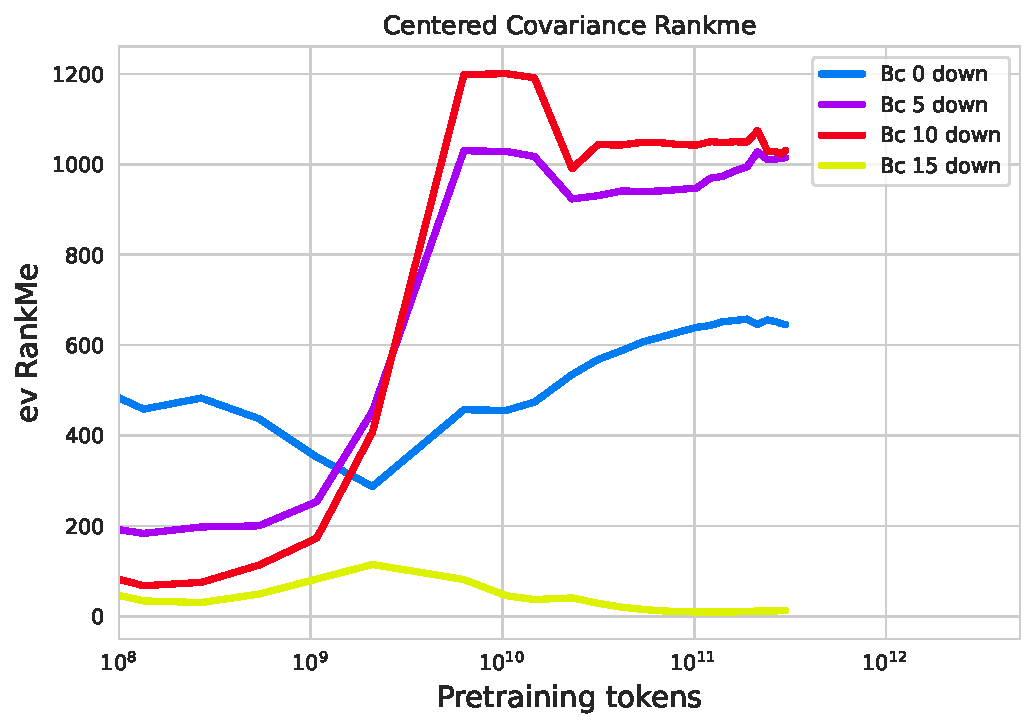
\includegraphics[width=\gridimg, trim=\cropL{} \cropBtop{} \cropR{} \cropT, clip]{attachments/mlp_down/py1b_rm_c.pdf} &  % trim:20,20,0,20
    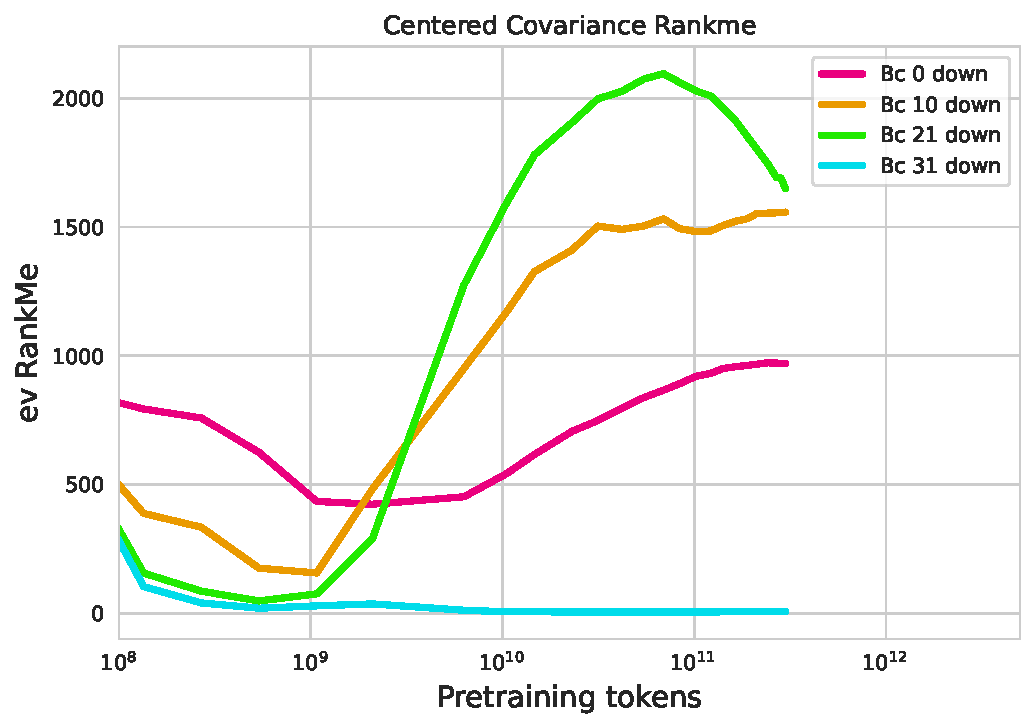
\includegraphics[width=\gridimg, trim=\cropL{} \cropBtop{} \cropR{} \cropT, clip]{attachments/mlp_down/py6.9b_rm_c.pdf} &   % trim:20,20,0,20
    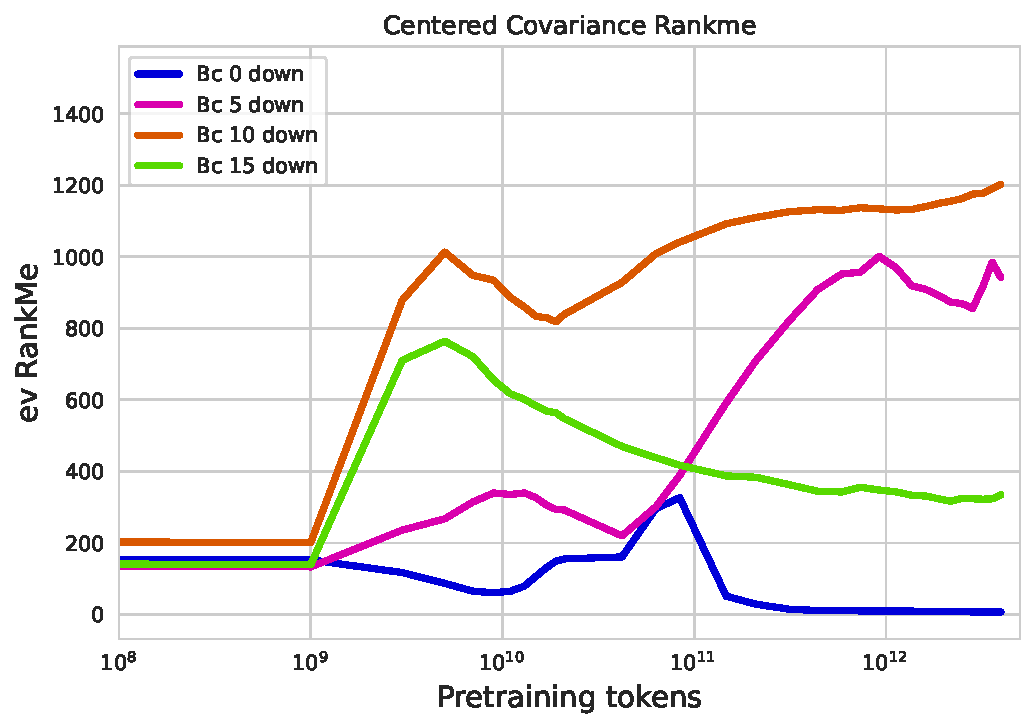
\includegraphics[width=\gridimg, trim=\cropL{} \cropBtop{} \cropR{} \cropT, clip]{attachments/mlp_down/ol1b_rm_c.pdf} &      % trim:20,20,0,20
    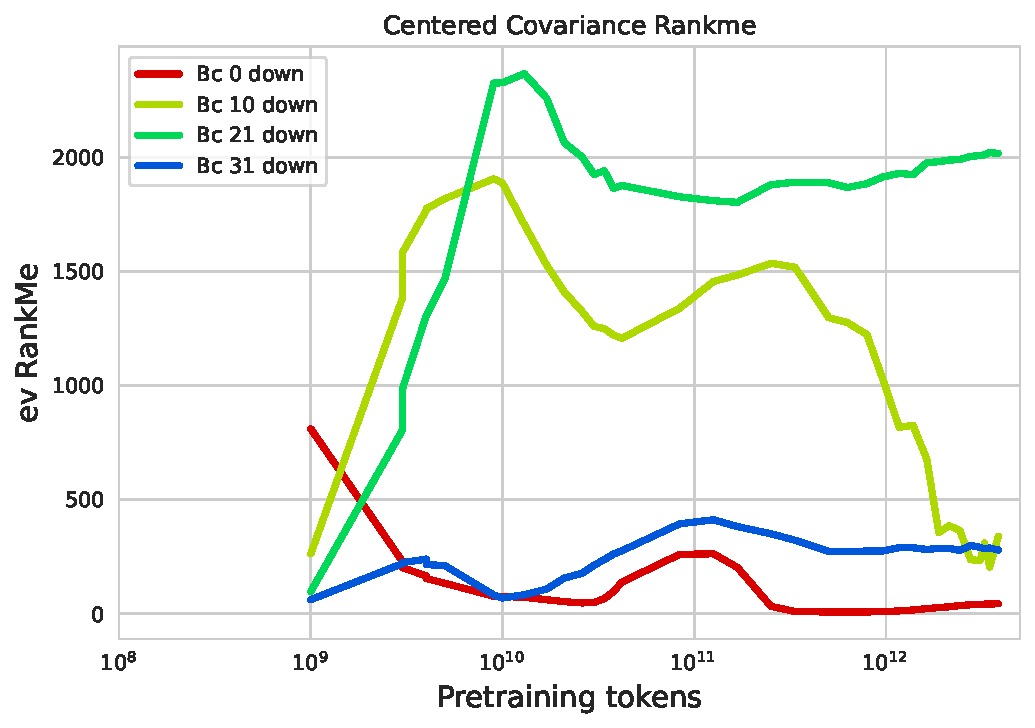
\includegraphics[width=\gridimg, trim=\cropL{} \cropBtop{} \cropR{} \cropT, clip]{attachments/mlp_down/ol7b_rm_c.pdf} \\[4pt] % trim:20,20,0,20
    \rotatebox{90}{\small\hspace{0.5em}\shortstack{Uncentered\\RankMe}} &
    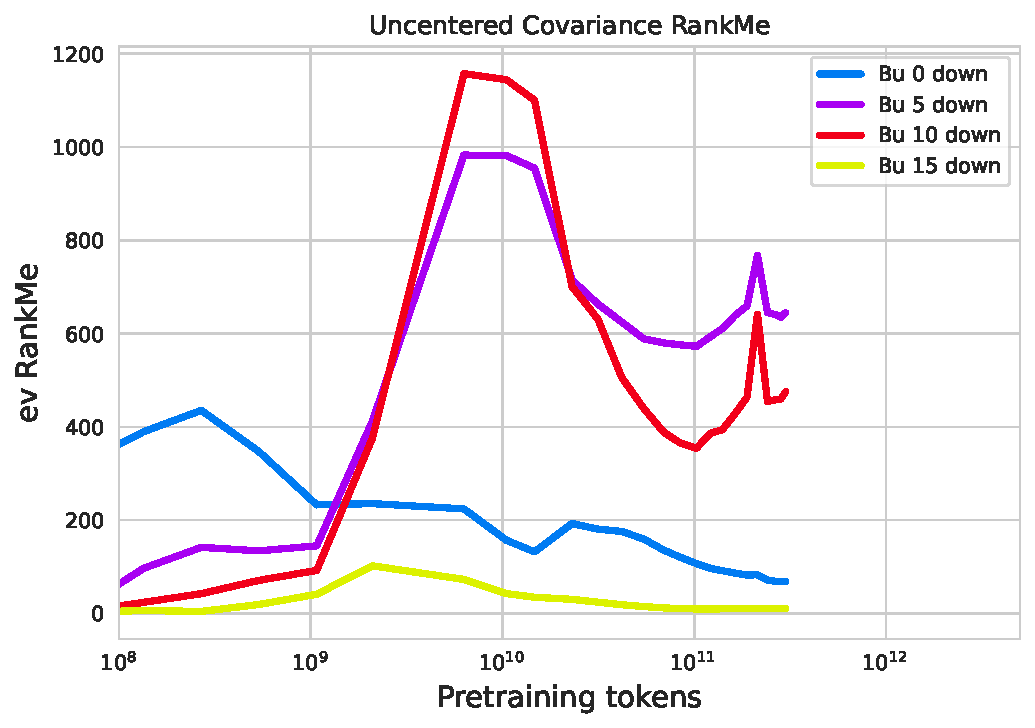
\includegraphics[width=\gridimg, trim=\cropL{} \cropB{} \cropR{} \cropT, clip]{attachments/mlp_down/py1b_rm_u.pdf} &  % trim:20,0,0,20
    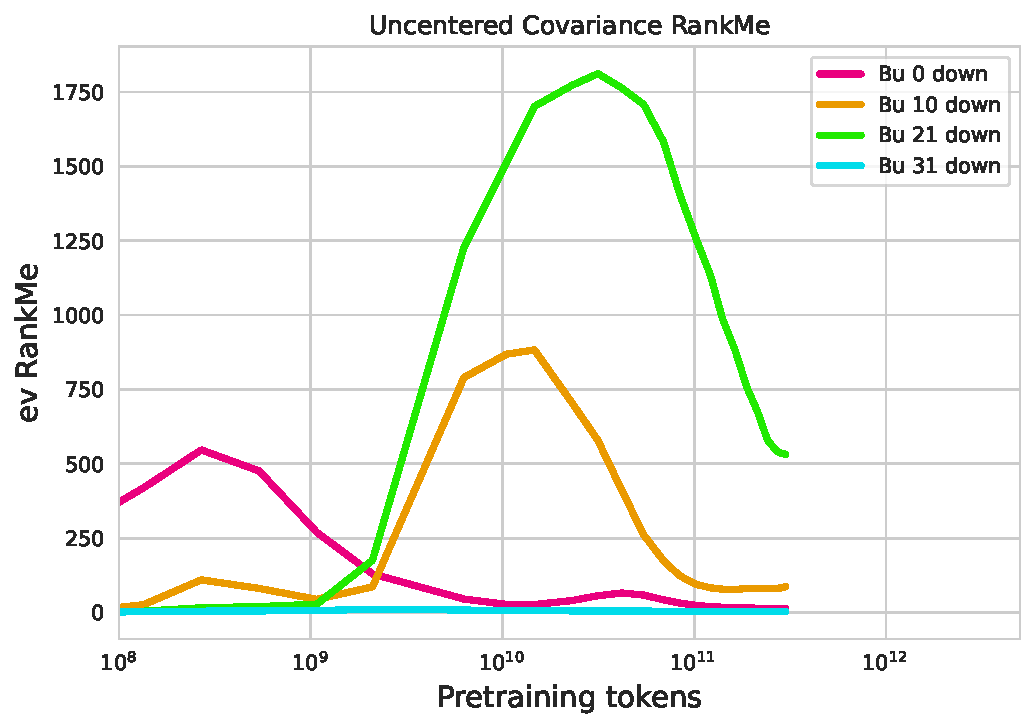
\includegraphics[width=\gridimg, trim=\cropL{} \cropB{} \cropR{} \cropT, clip]{attachments/mlp_down/py6.9b_rm_u.pdf} &   % trim:20,0,0,20
    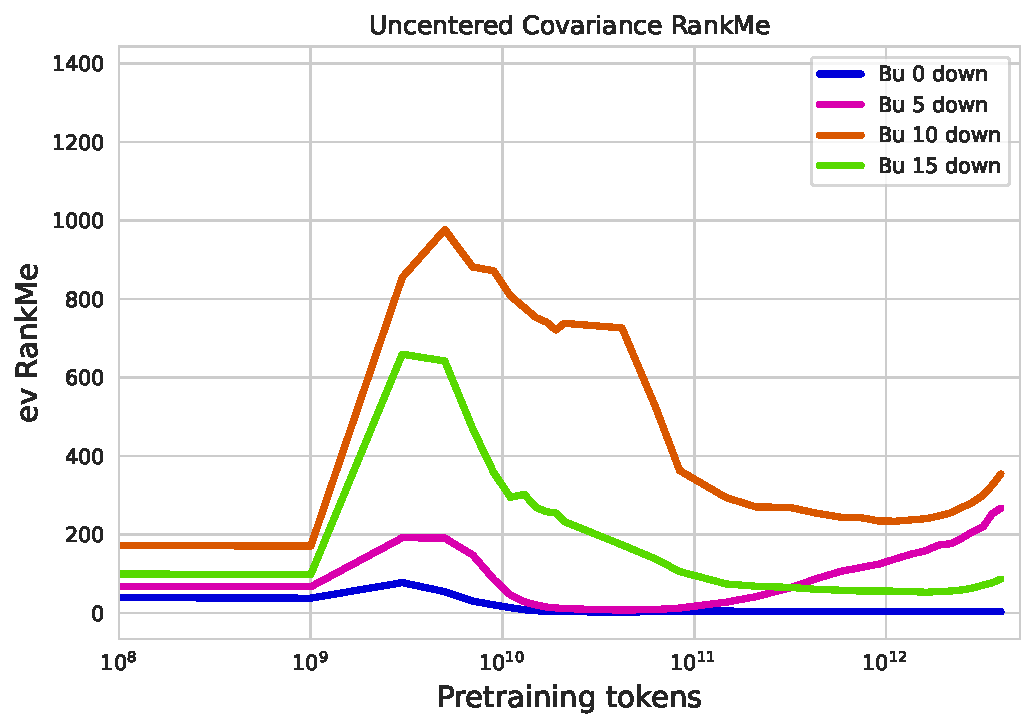
\includegraphics[width=\gridimg, trim=\cropL{} \cropB{} \cropR{} \cropT, clip]{attachments/mlp_down/ol1b_rm_u.pdf} &      % trim:20,0,0,20
    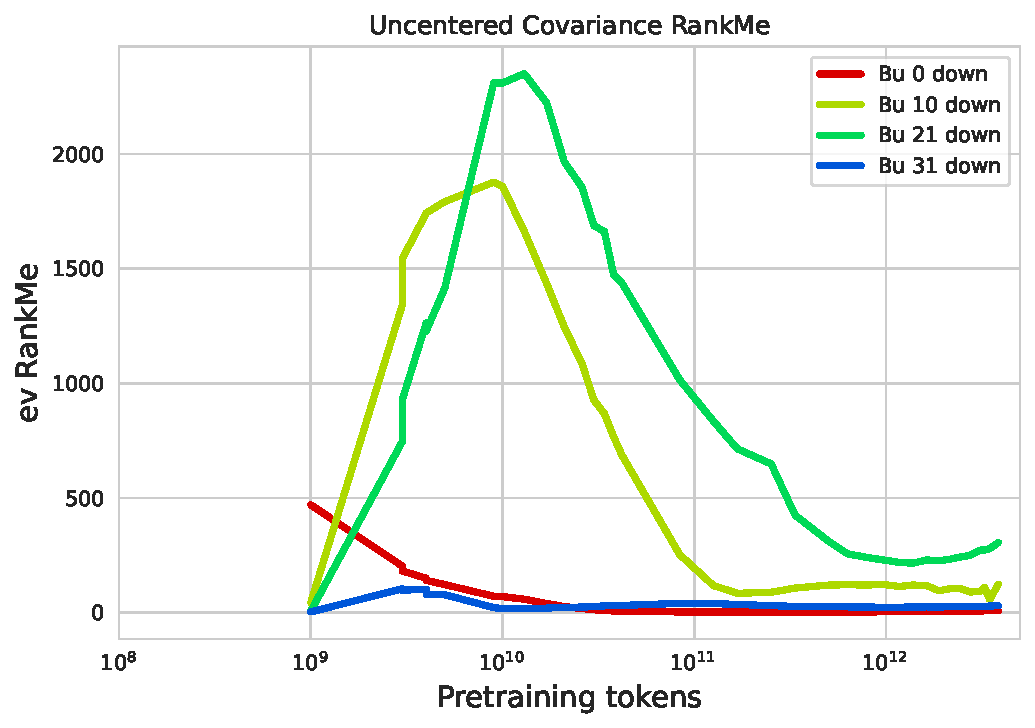
\includegraphics[width=\gridimg, trim=\cropL{} \cropB{} \cropR{} \cropT, clip]{attachments/mlp_down/ol7b_rm_u.pdf} \\      % trim:20,0,0,20
  \end{tabular}
  \caption{RankMe of MLP down-projection outputs over training.}
  \label{fig:rankme_grid}
\end{figure}

Most of the layers in most of the models do have a small dip, but it isn't as significant as the original compression seeking phase, and it is very short, after which the uncentered covariance stays mostly constant. Only layer OLMo-2 7B has one layer that really does compress strongly in the end, however, that is exactly the point at which the final residual actually starts to grow in entropy again. Interestingly, when we plot uncentered RankMe, we do see the compression-seeking phase. Indicating the mean is large enough to cause significant perceived compression. This is still in contrast to the final point of the residual stream, which shows a similar significant compression even when centered.

I hypothesise that the means of the intermediate layers do not align with each other or the mean of the residual. This then causes the first few directions of the residual to become the means of the layers.

Another observation, is that the activations at the first and last layers tend to have a significantly lower RankMe value than in the middle. For pythia models, we see this even more clearly at the input of the down-projection.

\begin{figure}[ht]
  \centering
  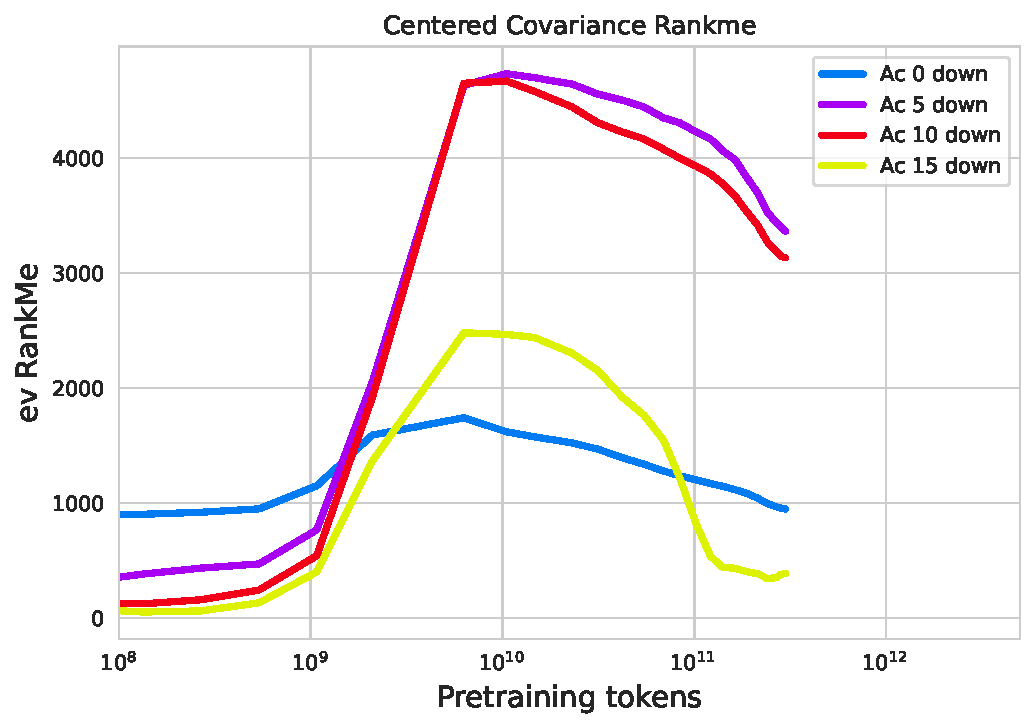
\includegraphics[width=0.48\linewidth]{attachments/mlp_down_in/py1b.pdf}
  \hfill
  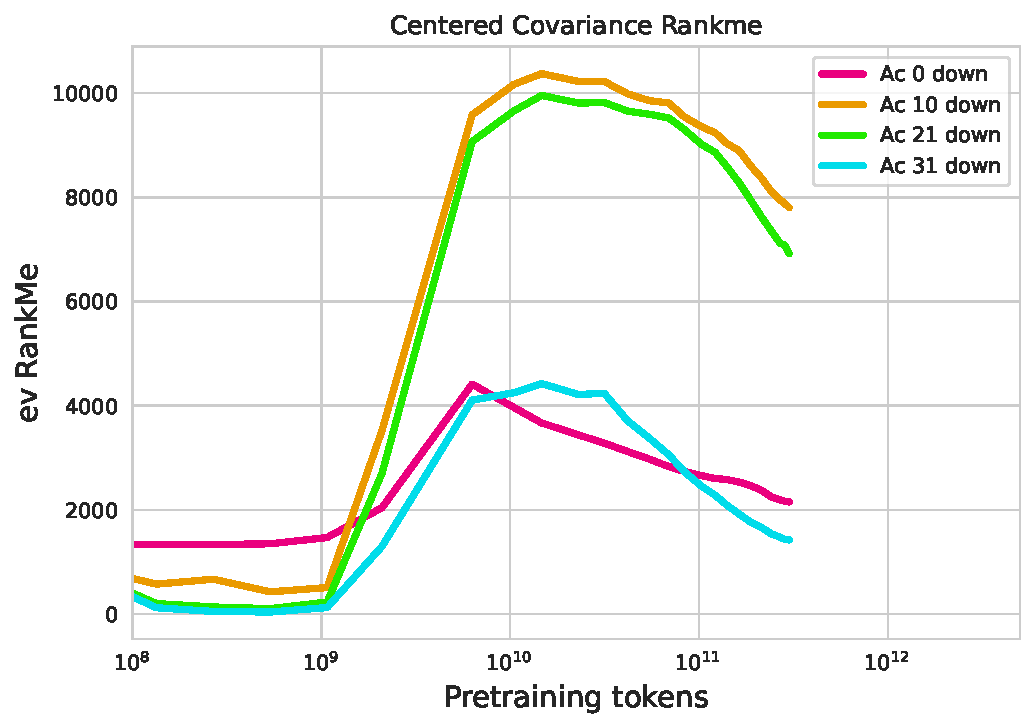
\includegraphics[width=0.48\linewidth]{attachments/mlp_down_in/py6.9b.pdf}
  \caption{RankMe of MLP down-projection inputs of pythia models over training. The first and last layers consistently have very low entropy relative to middle layers.}
  \label{fig:rankme_mlp_down}
\end{figure}

This is remarkable, because in literature, the middle layers often appear as a \emph{compression valley}. Although this tends to be associated with attention sinks and massive activations. However, because of the way we collect data, the likelihood of reading a BOS token is quite low. Additionally, the statement in literature that the middle layers appear to have low activations applies to the residual stream, not in the intermediate position of the MLPs.

\subsection{Other interesting activation covariance observations}

In the OLMo family, there is one part of training in which the layer 0 mean dominates the activation covariance. We measure at the input of the up-projection of the first layer. Pythia has a LayerNorm present before this exact hookpoint, so it may be nullified by that, yet still present before the LayerNorm. That must be tested separately.

\begin{figure}[ht]
  \centering
  \setlength{\tabcolsep}{2pt}
  \begin{tabular}{@{}cccc@{}}
    \small Pythia-1B & \small Pythia-6.9B & \small OLMo-2-1B & \small OLMo-2-7B \\[2pt]
    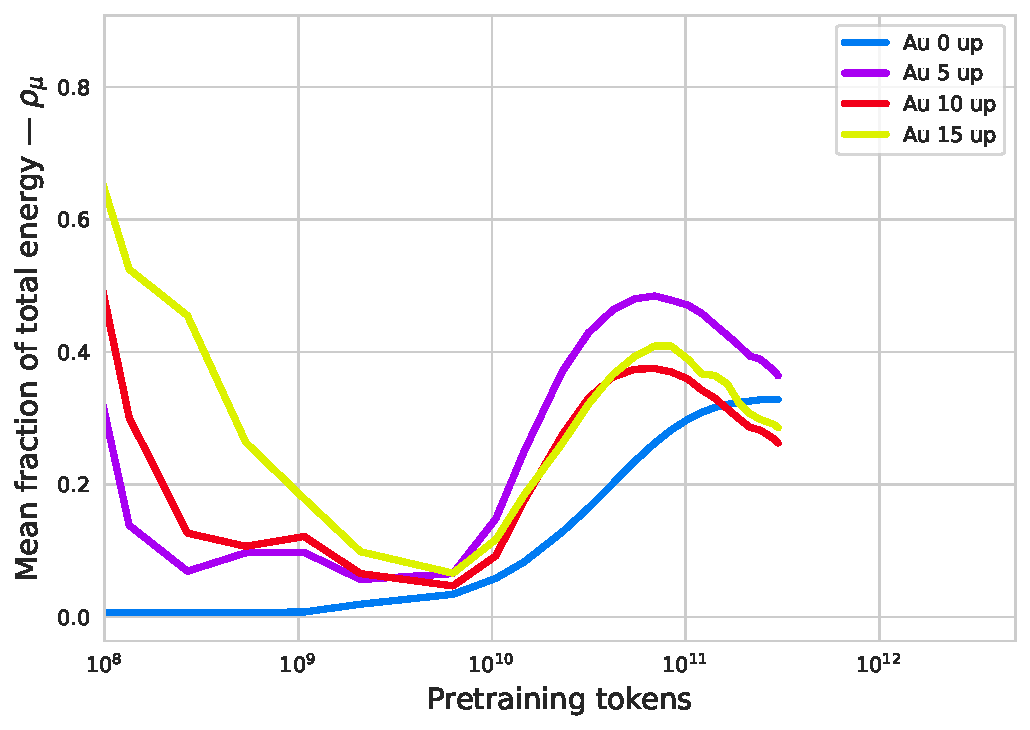
\includegraphics[width=0.24\linewidth]{attachments/layer0_mean/py1b.pdf} &
    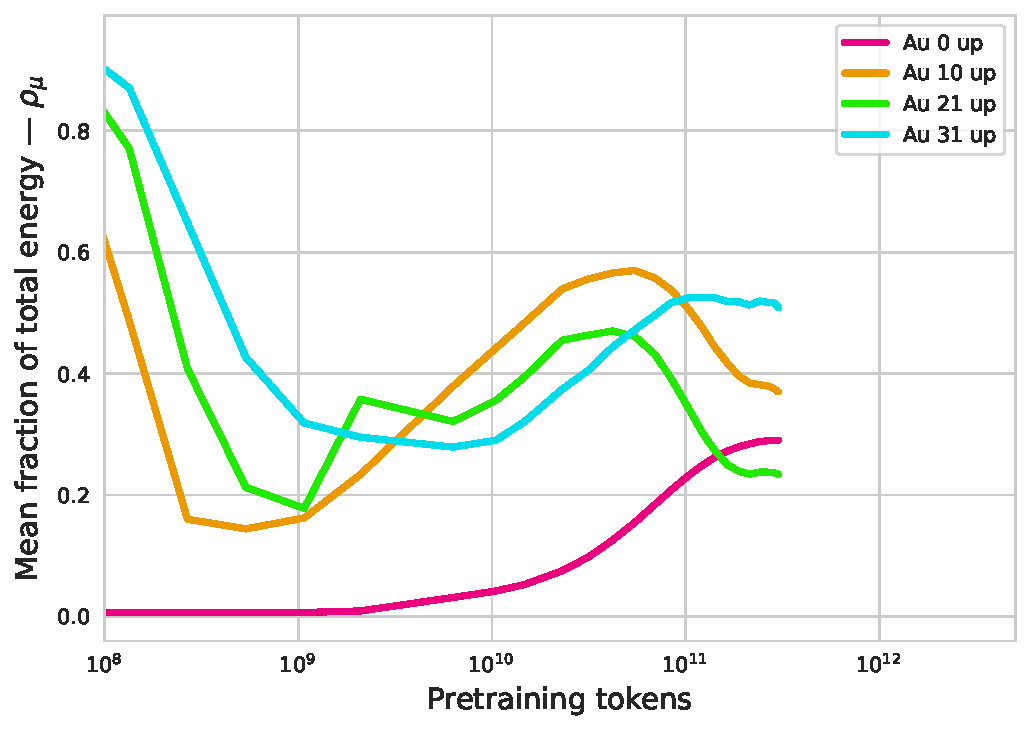
\includegraphics[width=0.24\linewidth]{attachments/layer0_mean/py6.9b.pdf} &
    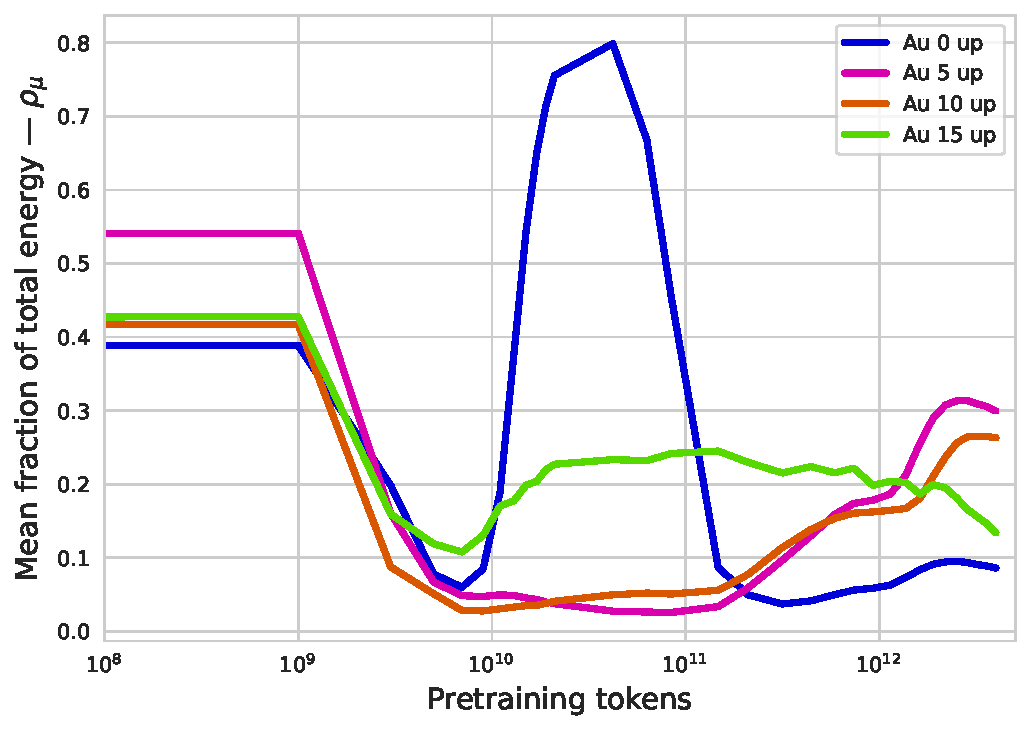
\includegraphics[width=0.24\linewidth]{attachments/layer0_mean/ol1b.pdf} &
    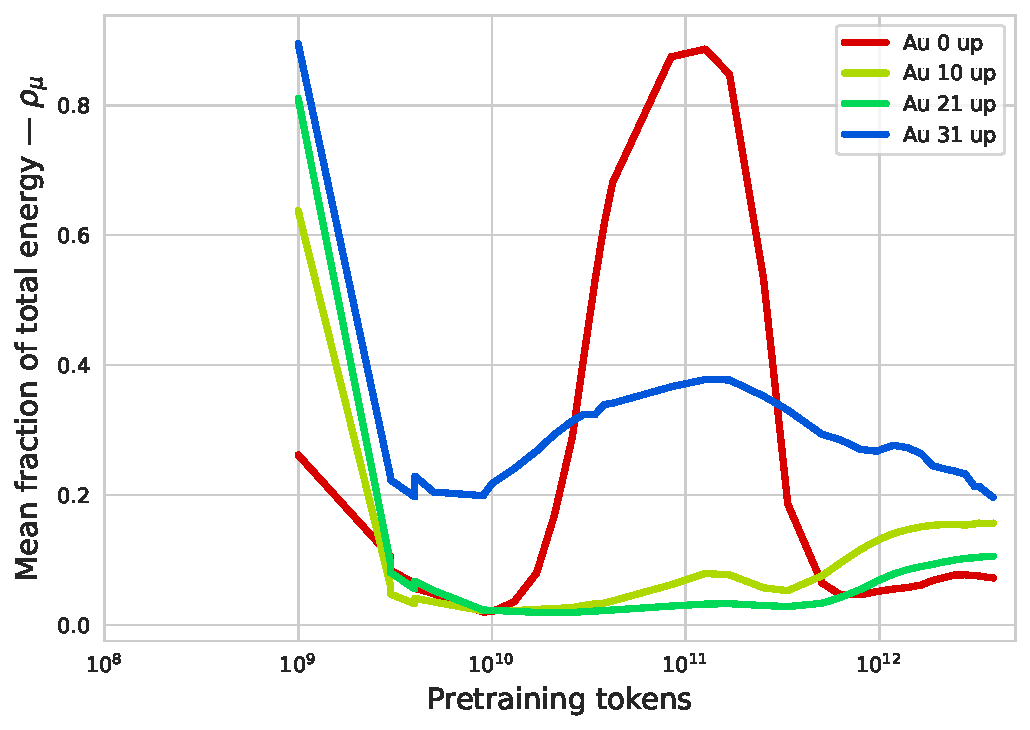
\includegraphics[width=0.24\linewidth]{attachments/layer0_mean/ol7b.pdf} \\
  \end{tabular}
  \caption{Mean fraction of total activation energy ($\rho_\mu$) at the MLP up-projection input over training, shown for selected layers. In OLMo, layer~0 exhibits a large transient mean-dominance peak.}
  \label{fig:layer0_mean}
\end{figure}

At first, it seems this is just the point at which the input-embedding learns the most common token, but oddly enough this peak happens quite late in training, around the start of the compression seeking phase. It starts growing shortly after the learning rate scheduler has finished warmup, but it lasts until surpringly long after.

\subsection{K-FAC of MLP weights}

We find that our K-FAC plots are in general difficult to interpret. The type of plot differs wildly by model family, likely in large due to differences in layernorm positioning and other architectural differences.

Here we show the log-determinants of the of the up-projections.

\begin{figure}[ht]
  \centering
  \setlength{\tabcolsep}{2pt}
  \begin{tabular}{@{}cccc@{}}
    \small Pythia-1B & \small Pythia-6.9B & \small OLMo-2-1B & \small OLMo-2-7B \\[2pt]
    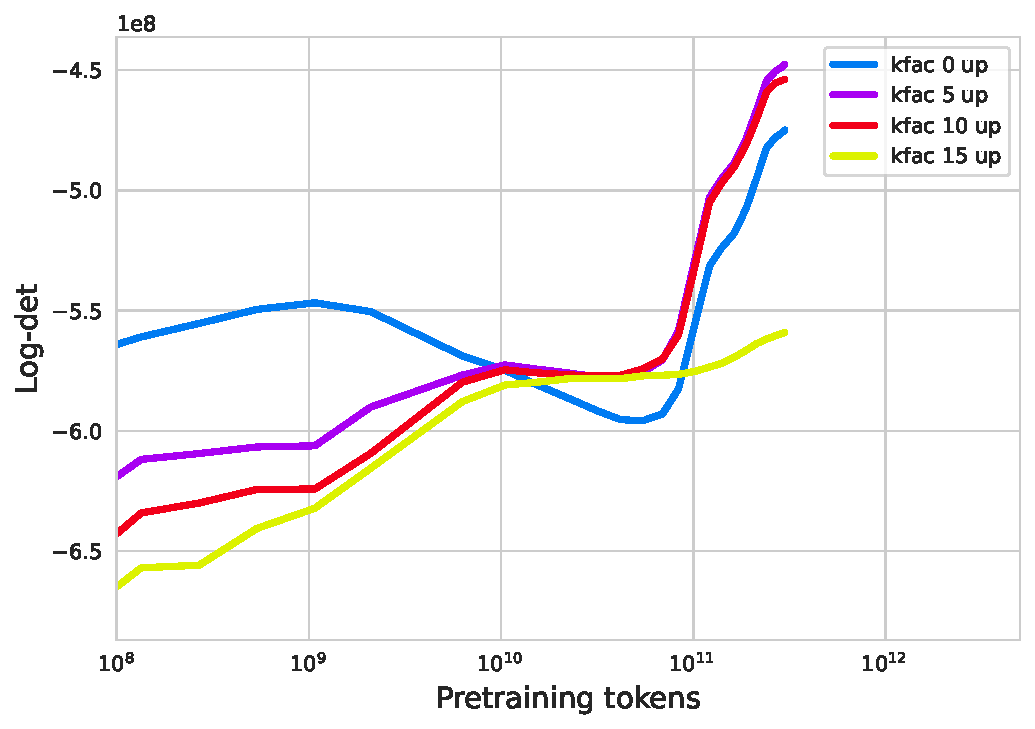
\includegraphics[width=0.24\linewidth]{attachments/kfac/py1b_up.pdf} &
    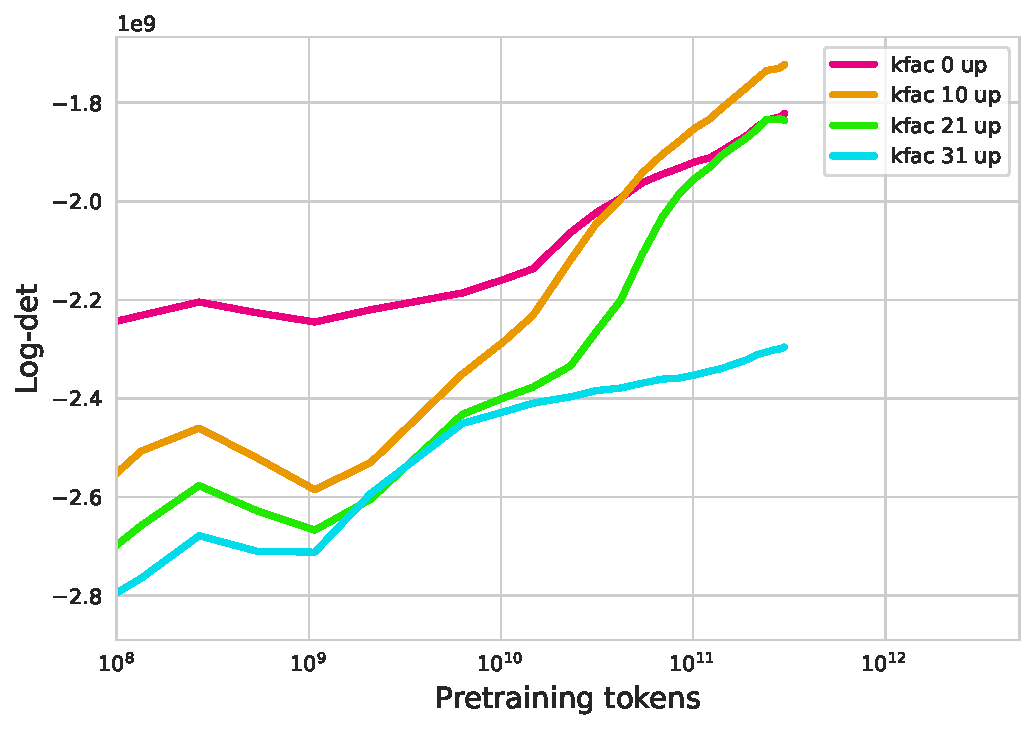
\includegraphics[width=0.24\linewidth]{attachments/kfac/py6.9b_up.pdf} &
    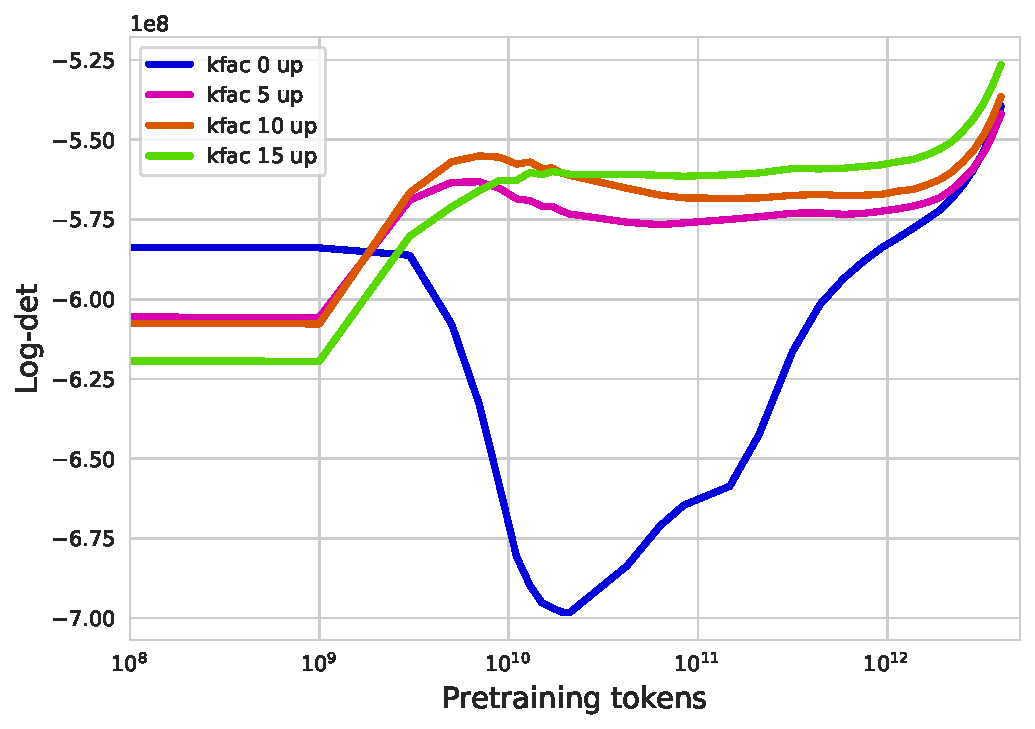
\includegraphics[width=0.24\linewidth]{attachments/kfac/ol1b_up.pdf} &
    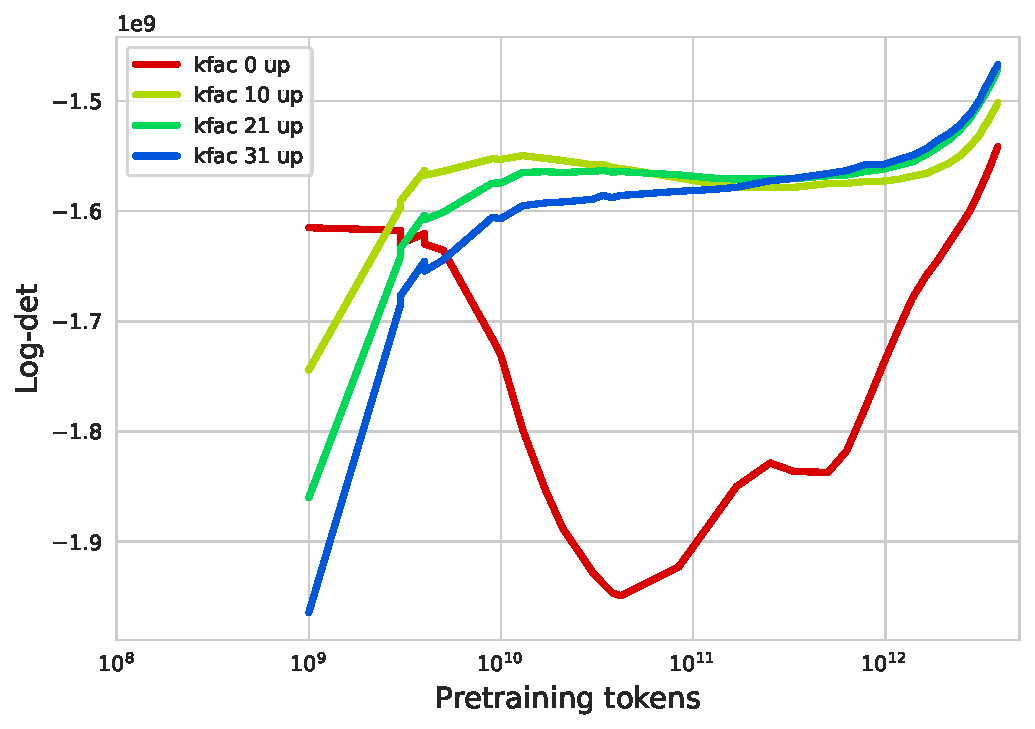
\includegraphics[width=0.24\linewidth]{attachments/kfac/ol7b_up.pdf} \\
  \end{tabular}
  \caption{K-FAC log-determinants of MLP up-projection covariance factors over training, shown for selected layers.}
  \label{fig:kfac_up}
\end{figure}

K-FAC also makes assumptions on model convergence. Meaning that training checkpoint values may not correctly represent curvature. The relationship between the Hessian and Fisher information is through the generalized Gauss-Newton decomposition:

$$ H = F + S $$

Where the Fisher information $F$ approximates the Hessian $H$ when the residual term $$S = \mathbb{E}_{x \sim p_{\text{data}}, y \sim p(y|x;\theta)} [\nabla^2 \log p(y|x;\theta)]$$ approaches zero. Unfortunately, during training this is never the case. Ideally, we at least approximate the size of our error term, but this is in itself also quite difficult.

The cheapest curvature measurement alternative that does not make the above assumption would be the Hutchinson Trace Estimator. It would also potentially be better to take the curvature with respect to the token labels as opposed to the model's intrinsic curvature, to both reduce variance and reframe the measurement in order to observe how the model weights respond to a new sample.

\section{What's next?}

In the following section, I present potential next steps, research questions, and ways to answer them.

\subsection{1. How the geometry phases form across layers}

In the findings, we saw that the entropy-seeking and compression-seeking phases show up cleanly at the final residual, but are largely absent from individual MLP outputs. This suggests the phases are emergent from the combination of layers rather than present in each one independently.

\subsubsection{Do the phases exist independently in each layer, or are they emergent from the combination of layers?}

Hypotheses contributing to answering this question:

\begin{itemize}
  \item \textbf{The phases emerge through combination.}

    Individual block outputs may not follow the phases themselves, but they form in the residual through constructive interference as block outputs are summed.
    \begin{notes}
      \item Maybe the MLP output mean, not its covariance, is what drives the residual's RankMe.
      \item I have strong evidence for this already. MLP uncentered RankMe drops through training while centered RankMe mostly does not.
      \item Subhypothesis: if a model used sub-layer post-norm with LayerNorm instead of RMSNorm, this probably wouldn't happen.
    \end{notes}
    \begin{experiments}
    \begin{itemize}
      \item Measure after the OLMo's block RMSNorm, not before.
      \item Measure how much the MLP output directions align with the residual's. Including the alignment of the mean.
      \item Measure more layers, including Attention. Compare the average output entropy of layers with the final entropy.
      \item Compare the attention block and mlp block output entropy, perhaps only one contributes to compression-seeking.
    \end{itemize}
    \end{experiments}
  \item \textbf{The phases are attributable to one type of layer more than others (MLP blocks or attention blocks).}
  \item \textbf{The phases do form within all layers, but only after some architectural element.}
\end{itemize}

If successful, this direction naturally leads towards looking at posttraining.

\subsection{2. Distinguishing maths from quotes}

Although the previous direction has potential to close some open questions. It might be difficult to tie those findings to downstream phenomena. Another direction lies in fixing the work of \citet{merullo2025memorization}, which unintentionally affects downstream maths performance. From this direction, we can study the geometric structure of the datasets, rather than studying the evolution of the model's geometry. This does however lead us quite orthogonally from our current results, but makes use of our data collection framework.

\subsubsection{Does maths or numerical data have more shared geometric structure than quotes or memorised data does?}

Hypotheses contributing to answering this question:

\begin{itemize}
  \item \textbf{In memorised data, gradient eigenstructure is uncorrelated with activations. In maths data, it is more correlated.}
    \begin{notes}
      \item  Medium confidence.
      \item To learn unstructured data, information attempts to be stored in any direction. To learn a shared mechanism, changes must be made to directions already used by other examples in the same task type.
    \end{notes}
    \begin{experiments}
    \begin{itemize}
      \item Prior step: to remove trivial, non-task-specific connections, subtract the general population's eigenspectrum from the task population's eigenspectrum.
      \item Check similarity between the SVDs of activations and gradients.
      \item Check properties of the spectrum obtained from a generalised eigenvalue problem with those SVDs.
    \end{itemize}
    \end{experiments}
  \item \textbf{Memorised spurious data does not share a common geometry beyond the general population's geometry, but in niche but logical data, there is a shared structure within the category that lies in the tail of the general population.}
    \begin{notes}
      \item High confidence.
      \item After accounting for the general population's structure present in most data, maths-like data still has common shared directions that are negligible in the general population, while memorisation has little additional structure.
    \end{notes}
    \begin{experiments}
    \begin{itemize}
      \item Check properties of the spectrum obtained from a generalised eigenvalue problem between the task and general populations.
      \item Check properties of the resorted eigenspectrum after subtracting the general population's eigenstructure from the task population's eigenstructure.
    \end{itemize}
    \end{experiments}
\end{itemize}

\subsubsection{Can we remove low-curvature K-FAC weight directions without affecting performance on niche non-memorisation tasks such as maths?}

Hypotheses contributing to answering this question:

\begin{itemize}
  \item \textbf{We can account for directions we want to keep by resorting the K-FAC components, factoring in the task-specific structure we don't want to remove.}
    \begin{notes}
      \item This is a hardcoded, non-general solution. Potential band-aids:
        \begin{itemize}
          \item Automate by accounting for any and all downstream tasks we care about.
          \item Use findings from the two research questions above to rate data sources by cohesion, and account only for those that have common structure. It is unrealistic on both points to do this for every possible useful type of data, but it is still an upgrade over hardcoding one specific source.
        \end{itemize}
    \end{notes}
    \begin{experiments}
    A K-FAC layer eigenvalue is the activation covariance component's eigenvalue multiplied by the gradient covariance component's eigenvalue. We could:
    \begin{itemize}
      \item Replace the basis (of activations or gradients) with another basis that accounts for task-specific structure.
      \item Leave the original bases in place, but project another eigenbasis with its eigenvectors onto them to obtain new eigenvalues that are only used for sorting.
    \end{itemize}
    \end{experiments}
\end{itemize}

\begin{weboptional}{3. Annoying unknowns that may still be worth investigating}
\subsubsection{Why do middle-layer MLPs have \emph{higher} entropy than the first or last layer?}

This is the opposite of the typical ``compression valleys'' phenomenon in the literature, where middle layers are reported to have low entropy.

\begin{itemize}
  \item We mask the first 30 tokens, which are the positions most likely to contain the BOS token. BOS is a common attention sink and massive activation.
  \item The last layer may have prediction-specific properties, based on evidence from my token-space analysis with the entropy-lens.
\end{itemize}

\subsubsection{Why are some of our results different from \texorpdfstring{\citet{li2025tracing}}{Li et al.\ (2025)}?}

\begin{itemize}
  \item On the fineweb RankMe being consistently somewhat lower than theirs:
    \begin{itemize}
      \item Perhaps different dataloading.
      \item Perhaps they normalise.
    \end{itemize}
  \item On the per-layer RankMe:
    \begin{itemize}
      \item Most likely Pythia's prenorm sits before our hook, so we aren't really measuring the residual stream.
      \item Potentially all-token selection vs last-token selection.
    \end{itemize}
\end{itemize}
\end{weboptional}




% =========================================================
\bibliographystyle{plainnat}
\bibliography{citations}
% =========================================================

\end{document}
